\documentclass[aspectratio=169,usenames,dvipsnames]{beamer}
\beamertemplatenavigationsymbolsempty
% \documentclass{beamer}

% UNCOMMENT FOR HANDOUTS
% \usepackage{pgfpages}
% \pgfpagesuselayout{2 on 1}[landscape,letterpaper,border shrink=5mm]
% \setbeameroption{show notes}

\mode<presentation>
\usetheme{Boadilla}
\usecolortheme{spruce}
\usepackage{../../LizStyle,ulem}
\usepackage{color}
\usepackage[color,matrix,arrow]{xy}
% \input xy
% \xyoption{all}
\usepackage{tikz}
\usepackage{tikz-cd}
\tikzset{commutative diagrams/diagrams={ampersand replacement=\&}}

\AtBeginSection{\frame{\sectionpage}}


% ==========Command for putting comments and removing them=======
% Visible:
\newcommand{\InstructorNotes}[1]{\textit{\color{orange}#1}}
\newcommand{\InstructorList}[1]{
\begin{itemize}
	\color{orange}
	#1
\end{itemize}
}
% Removed:
% \renewcommand{\InstructorNotes}[1]{}
% \renewcommand{\InstructorList}[1]{}


\newcommand{\bvfill}{\vskip0pt plus 1filll}

\usepackage{multimedia}
\usepackage{graphbox}

% \usepackage{algpseudocode}


\newcommand{\Reeb}{\textbf{Reeb}}
\newcommand{\Rtopc}{\textbf{Rtopc}}
% \newcommand{\RR}{\mathcal{R}}

\newcommand{\Set}{\textbf{Set}}
\newcommand{\Vect}{\textbf{Vect}}
\newcommand{\Top}{\textbf{Top}}
\newcommand{\Int}{\textbf{Int}}


\graphicspath{ {Figures/} {../Figures/}{../../Figures/} }



\begin{document}
%\pdfoptionpdfminorversion 5
%\logo{\includegraphics[height=1.5cm]{dukeshield.pdf}}
\title[]{Ch 6.1: Subset Selection}
\subtitle{Lecture 16 - CMSE 381}
\date{Mon, Feb 23, 2026}



\institute[MSU-CMSE]{Michigan State University\\
			::\\
          Dept of Computational Mathematics, Science \& Engineering}


\begin{frame}
 \titlepage


\end{frame}
%--------------------------
\begin{frame}[c]{Announcements}

\begin{columns}
\column{.45\textwidth}
\centering

\textbf{Last time}
\begin{itemize}
	\item $k$-fold CV for Classification
\end{itemize}
	\textbf{Covered in this lecture}
\begin{itemize}
	% \item response to feedback (from Quiz 5)
	\item Subset selection
	\item Forward and Backward Selection
	% \item Adjusted training MSE scores: $C_p$, AIC, BIC, Adjusted $R^2$ % Removed this 2023 cuz I just hate it.

\end{itemize}
\textbf{Announcements:}
	\begin{itemize}
		\item HW \#4 due Sunday 3/8
		\item HW \#5 due Sunday 3/15
	\end{itemize}
\column{.45\textwidth}
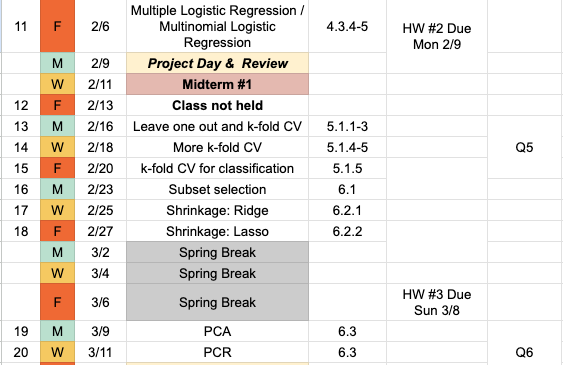
\includegraphics[align = c, width = \textwidth]{Schedule-S26-Lecs11_to_20}
\centering

\end{columns}
\bvfill 


\end{frame}

% %--- Next Frame ---%
% \begin{frame}[t]{Feedback collected in Quiz 5}
% 	\begin{itemize}
% 		\item what I can do:
% 		\begin{itemize}
% 			\item I will add overview slide at the beginning of each lecture. This will become a study guide for the exam.  
% 			\item I will provide you a practice exam with matched difficulty. Those questions will not be in the exam.
% 			\item Code portfolios as bonus assignments. I will provide a template. 
% 		\end{itemize}
% 		\item what you can do:
% 		\begin{itemize}
% 			\item Take better notes
% 			\item Read the textbook (read before class if you have trouble following the lecture)
% 			\item Ask more questions (in class, on slack, office hours/helproom) and respond to the review class ``burning questions'' survey
% 		\end{itemize}
% 	\end{itemize}
% \end{frame}

%--- Next Frame ---%
\begin{frame}[t]{What should you learn from this lecture?}
	\begin{itemize}
		\item Why shouldn't you have as many predictors in your model as possible? 
		\item What are the three basic methods could be used to select the appropriate predictors (feature selection)? 
		\item What are the steps/procedures in the algorithm for each of these methods? 
		\item How to implement these procedures by hand given the training and CV test error for each combo of predictors? 
		\item What are the pros and cons for choosing each of these feature selection methods? When you can or cannot use them?
		\item How do you implement the feature selection algorithm in Python?
	\end{itemize}
\end{frame}
%--- Next Frame ---%
%=================
\section{Previously on linear regression ...}
%=================

\begin{frame}[t]{The problem of many features (p) relative to samples (n)}
	Up to now, we've focused on standard linear model:
	% \begin{equation*}
		$Y = \beta_0 + \beta_1 X_1 + \cdots + \beta_p X_p + \e$
	% \end{equation*}
	and done least squares estimation.
	\InstructorNotes{Translation: Minimize $RSS = \sum_{i}(y_i-\hat y_i)^2$}
\begin{columns}
\column{.45\textwidth}
\centering
\textbf{Prediction accuracy}
\footnotesize
\InstructorList{
\item If the true relationship is approximately linear, least squares estimates have low bias
\item If $n \gg p$, then least squares also has low variance
\item If $n$ not much larger than $p$, then high variability, overfitting, poor predictions
\item If $n<p$ then no unique solution so can't use at all
\item Goal on next slide: shrink/constrain number of variables to improve accuracy
}
\column{.45\textwidth}
\centering
% \textbf{Model Interpretability}
% \footnotesize
% \InstructorList{
% \item Often, many variables included aren't associated with response
% \item Including them leads to unnecessary complexity in the model
% \item Idea: Set these coefficients to 0 (or close to zero)
% \item Goal on next slide: Do some automatic feature selection / variable selection to get rid of unnecessary variables
% }
\end{columns}

\end{frame}
%--- Next Frame ---%
\begin{frame}[t]{The problem of many features (p) relative to samples (n)}
	Up to now, we've focused on standard linear model:
	% \begin{equation*}
		$Y = \beta_0 + \beta_1 X_1 + \cdots + \beta_p X_p + \e$
	% \end{equation*}
	and done least squares estimation.
	\InstructorNotes{Translation: Minimize $RSS = \sum_{i}(y_i-\hat y_i)^2$}
\begin{columns}
	\column{.45\textwidth}
	\centering


\textbf{Model Interpretability}
\footnotesize
\InstructorList{
\item Often, many variables included aren't associated with response
\item Including them leads to unnecessary complexity in the model
\item Idea: Set these coefficients to 0 (or close to zero)
\item Goal on next slide: Do some automatic feature selection / variable selection to get rid of unnecessary variables
}
\column{.45\textwidth}
\centering
\end{columns}

\end{frame}
%--- Next Frame ---%
% \begin{frame}[c]{Goal of next chapter}

% \begin{columns}
% \column{.45\textwidth}
% \centering
% % Use something other than least squares to fit:

% \InstructorNotes{Classes of methods }
% \InstructorList{
% \item Subset selection: identify subset of predictors, fit model using least squares on smaller set of variables
% \item Shrinkage:
% \InstructorList{
% \item Estimated coeff are shrunken towards zero relative to the least squares estimate
% }
% \item Dimension reduction: Project the $p$-dimensional data into $M$-dimensional subspace, $M <p$. Likely after the midterm.
% }
% \column{.45\textwidth}
% \centering

% \end{columns}

% \end{frame}
% %--- Next Frame ---%

%==========
\section{Best Subset Selection}
%==========
\begin{frame}[c]{Go through each combo of variables exhaustively (exhausting?)}

	\centering
All subsets of 4 variables ($2^4 = 16$)

\begin{columns}
\column{.2\textwidth}
\centering
\begin{itemize}
	\item $\emptyset$
\end{itemize}
\column{.2\textwidth}
\centering

\begin{itemize}
	\item $X_1$
	\item $X_2$
	\item $X_3$
	\item $X_4$
\end{itemize}
\column{.2\textwidth}
\centering
\begin{itemize}
	\item $X_1$ $X_2$
	\item $X_1$ $X_3$
	\item $X_1$ $X_4$
	\item $X_2$ $X_3$
	\item $X_2$ $X_4$
	\item $X_3$ $X_4$
\end{itemize}
\column{.2\textwidth}
\centering
\begin{itemize}
	\item $X_1$ $X_2$ $X_3$
	\item $X_1$ $X_2$ $X_4$
	\item $X_1$ $X_3$ $X_4$
	\item $X_2$ $X_3$ $X_4$
\end{itemize}
\column{.2\textwidth}
\centering
\begin{itemize}
	\item $X_1$ $X_2$ $X_3$ $X_4$
\end{itemize}
\end{columns}

\InstructorList{
	\item The game: fit the model $2^n$ times, score each, pick one with best score
	\item point out this is tiered by number of variables (k) out of p variables
	\item easy to compare model with the same k (no order difference) 
	\item after come back from next slide: each tier has p choose k combos $\binom{p}{k} = \dfrac{p!}{k!(p-k)!}$
}
\end{frame}
%--- Next Frame ---%

\begin{frame}[c]{One way of breaking this up}

\begin{columns}
\column{.65\textwidth}
\centering
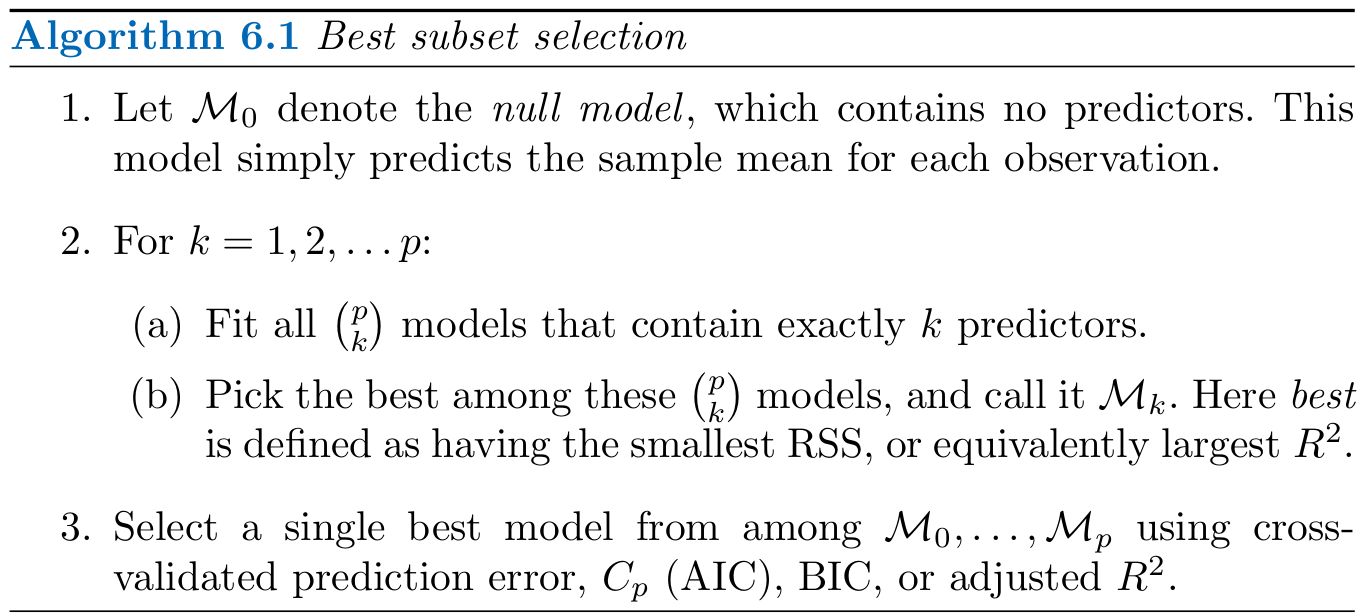
\includegraphics[width = \textwidth, align = c]{Alg6-1}

\end{columns}
\InstructorList{
\item Part 2b goes for lowest training score, Part 3 then goes for lowest testing score.
\item Go back to previous page and walk through the algorithm and variables slowly
\item point out that Step 2 is computational infeasable for large $p$
}
\end{frame}
%--- Next Frame ---%




\begin{frame}[t]{Calculate by hand }
We train a model using four variables, $X_1,X_2,X_3,X_4$.
We're interested in getting a subset of the variables to use. The following table shows the mean squared error and the MSE value computed for the model learned using each possible subset of variables.
\begin{columns}
\column{.45\textwidth}
\centering
% \begin{wrapfigure}{r}{1in}
\begin{center}
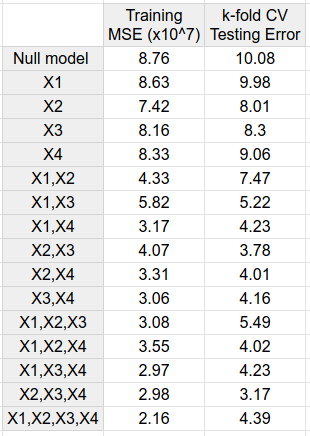
\includegraphics[width = .5\textwidth]{FakeData-SubsetSelection.png}
\end{center}
% \end{wrapfigure}

\column{.45\textwidth}
\centering
\begin{enumerate}
  \item What subset of variables is found for each of the sets $\mathcal{M}_0,\mathcal{M}_1,\mathcal{M}_2,\mathcal{M}_3,\mathcal{M}_4$ when using best subset selection?
\vfill
  \item What subset of variables is returned using best subset selection?

\vfill
%   \item What subset of variables is found for each of the sets $\mathcal{M}_0,\mathcal{M}_1,\mathcal{M}_2,\mathcal{M}_3,\mathcal{M}_4$ when using forward selection?
% \vfill
%   \item What subset of variables is returned using forward subset 
% \vfill
\end{enumerate}

\end{columns}
\end{frame}
%--- Next Frame ---%
\begin{frame}[t]{Extra work space if it helps}
\begin{columns}
\column{.25\textwidth}
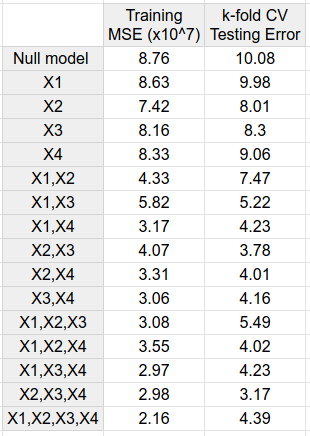
\includegraphics[width = \textwidth]{FakeData-SubsetSelection.png}

\centering
\column{.1\textwidth}
\centering
\begin{itemize}
	\item $\emptyset$
\end{itemize}
\column{.1\textwidth}
\centering

\begin{itemize}
	\item $X_1$
	\item $X_2$
	\item $X_3$
	\item $X_4$
\end{itemize}
\column{.15\textwidth}
\centering
\begin{itemize}
	\item $X_1$ $X_2$
	\item $X_1$ $X_3$
	\item $X_1$ $X_4$
	\item $X_2$ $X_3$
	\item $X_2$ $X_4$
	\item $X_3$ $X_4$
\end{itemize}
\column{.15\textwidth}
\centering
\begin{itemize}
	\item $X_1$ $X_2$ $X_3$
	\item $X_1$ $X_2$ $X_4$
	\item $X_1$ $X_3$ $X_4$
	\item $X_2$ $X_3$ $X_4$
\end{itemize}
\column{.2\textwidth}
\centering
\begin{itemize}
	\item $X_1$ $X_2$ $X_3$ $X_4$
\end{itemize}
\end{columns}
\InstructorNotes{
$
\mathcal{M}_0 = \emptyset,
\mathcal{M}_1 = \{X_2\},\,
\mathcal{M}_2= \{X_3,X_4\},\,
\mathcal{M}_3= \{X_1,X_3,X_4\},\,
\mathcal{M}_4 = \{X_1,X_2,X_3,X_4\},\,$.\\
 Among test error, best is  $X_3X_4$}
\end{frame}
%--- Next Frame ---%
{
\setbeamercolor{background canvas}{bg=Apricot!25}
\begin{frame}[t]{Code to do this}
\begin{columns}
\column{.45\textwidth}
\centering
\column{.45\textwidth}
\centering
\end{columns}
\end{frame}
}
%--- Next Frame ---%
%==========
\section{Forward Selection}
%==========



%--- Next Frame ---%
\begin{frame}[c]{What's the problem with best subset selection?}

\begin{columns}
\column{.45\textwidth}
\centering

\InstructorList{
\item Checking $2^p$ models is not reasonable for large $p$, $p >40$
\item The next bits are finding alternatives to Step 2
}
% \item as number of variables increases, RSS decreases and $R^2$ increases, so this is a bit of a problem
\column{.45\textwidth}
\centering

\end{columns}

\end{frame}
%--- Next Frame ---%

\begin{frame}[c]{Forward Stepwise Selection}

\begin{columns}
\column{.65\textwidth}
\centering
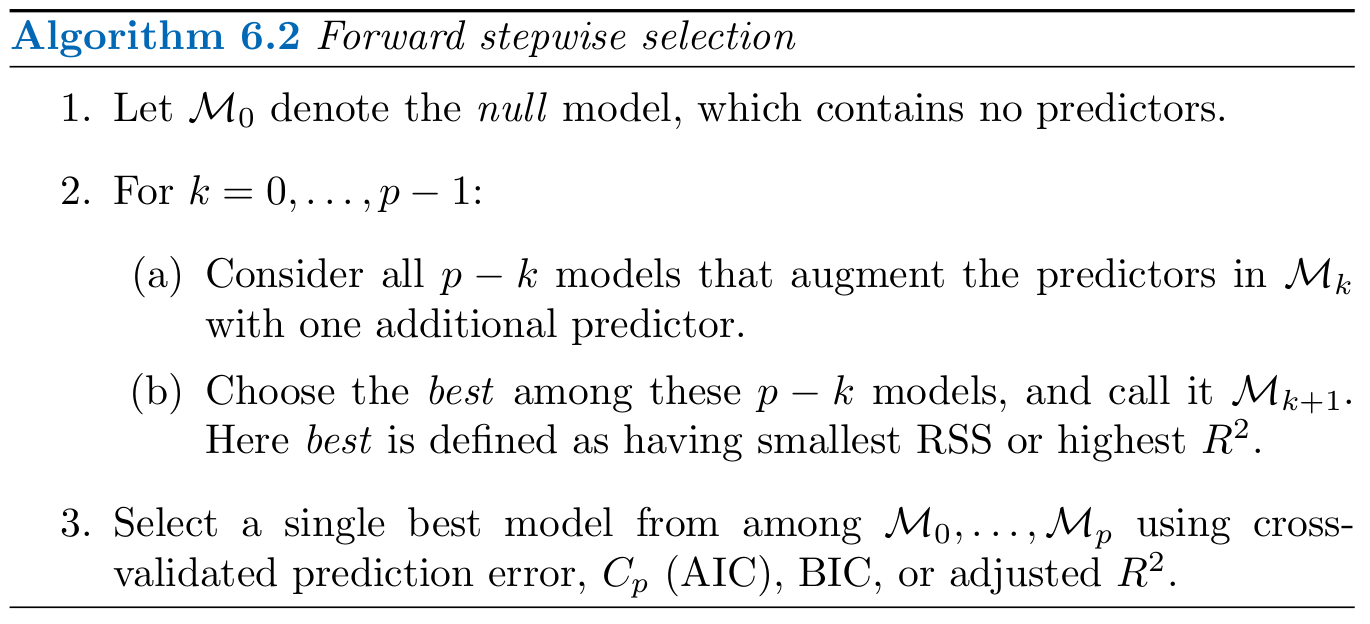
\includegraphics[width = \textwidth, align = c]{Alg6-2}

\end{columns}

\end{frame}
%--- Next Frame ---%

\begin{frame}[c]{An example for Forward Stepwise Selection}

	\centering
% All subsets of 4 variables ($2^4 = 16$)

\begin{columns}
\column{.2\textwidth}
\centering
\begin{itemize}
	\item $\emptyset$
\end{itemize}
\column{.2\textwidth}
\centering

\begin{itemize}
	\item $X_1$
	\item $X_2$
	\item $X_3$
	\item $X_4$
\end{itemize}
\column{.2\textwidth}
\centering
\begin{itemize}
	\item $X_1$ $X_2$
	\item $X_1$ $X_3$
	\item $X_1$ $X_4$
	\item $X_2$ $X_3$
	\item $X_2$ $X_4$
	\item $X_3$ $X_4$
\end{itemize}
\column{.2\textwidth}
\centering
\begin{itemize}
	\item $X_1$ $X_2$ $X_3$
	\item $X_1$ $X_2$ $X_4$
	\item $X_1$ $X_3$ $X_4$
	\item $X_2$ $X_3$ $X_4$
\end{itemize}
\column{.2\textwidth}
\centering
\begin{itemize}
	\item $X_1$ $X_2$ $X_3$ $X_4$
\end{itemize}
\end{columns}
\end{frame}
%--- Next Frame ---%
{
\setbeamercolor{background canvas}{bg=Apricot!25}
\begin{frame}[t]{Group work: by hand same example with forward example}
We train a model using four variables, $X_1,X_2,X_3,X_4$.
We're interested in getting a subset of the variables to use. The following table shows the mean squared error and the $R^2$ value computed for the model learned using each possible subset of variables.
\begin{columns}
\column{.45\textwidth}
\centering
% \begin{wrapfigure}{r}{1in}
\begin{center}
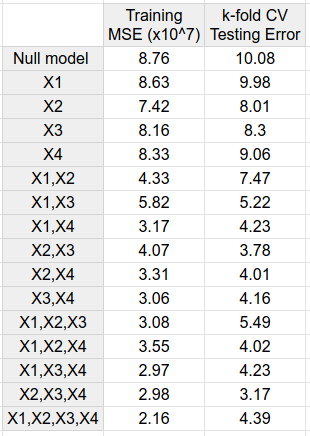
\includegraphics[width = .5\textwidth]{FakeData-SubsetSelection.png}
\end{center}
% \end{wrapfigure}

\column{.45\textwidth}
\centering
\begin{enumerate}
%   \item What subset of variables is found for each of the sets $\mathcal{M}_0,\mathcal{M}_1,\mathcal{M}_2,\mathcal{M}_3,\mathcal{M}_4$ when using best subset selection?
% \vfill
%   \item What subset of variables is returned using best subset selection?

% \vfill
  \item What subset of variables is found for each of the sets $\mathcal{M}_0,\mathcal{M}_1,\mathcal{M}_2,\mathcal{M}_3,\mathcal{M}_4$ when using forward selection?
\vfill
  \item What subset of variables is returned using forward subset selection?
\vfill
\end{enumerate}

\end{columns}
\end{frame}
}
%--- Next Frame ---%
{
\setbeamercolor{background canvas}{bg=Apricot!25}
\begin{frame}[t]{Extra work space if it helps}
\begin{columns}
\column{.25\textwidth}
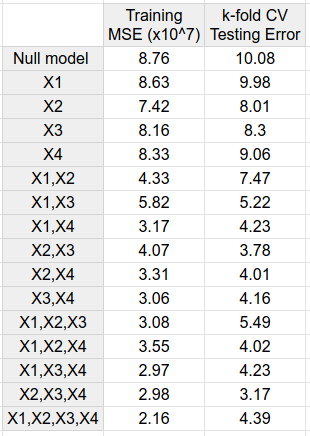
\includegraphics[width = \textwidth]{FakeData-SubsetSelection.png}

\centering
\column{.1\textwidth}
\centering
\begin{itemize}
	\item $\emptyset$
\end{itemize}
\column{.1\textwidth}
\centering

\begin{itemize}
	\item $X_1$
	\item $X_2$
	\item $X_3$
	\item $X_4$
\end{itemize}
\column{.15\textwidth}
\centering
\begin{itemize}
	\item $X_1$ $X_2$
	\item $X_1$ $X_3$
	\item $X_1$ $X_4$
	\item $X_2$ $X_3$
	\item $X_2$ $X_4$
	\item $X_3$ $X_4$
\end{itemize}
\column{.15\textwidth}
\centering
\begin{itemize}
	\item $X_1$ $X_2$ $X_3$
	\item $X_1$ $X_2$ $X_4$
	\item $X_1$ $X_3$ $X_4$
	\item $X_2$ $X_3$ $X_4$
\end{itemize}
\column{.2\textwidth}
\centering
\begin{itemize}
	\item $X_1$ $X_2$ $X_3$ $X_4$
\end{itemize}
\end{columns} 
\InstructorNotes{
$
\mathcal{M}_0 = \emptyset,
\mathcal{M}_1 = \{X_2\},\,
\mathcal{M}_2= \{X_2,X_4\},\,
\mathcal{M}_3= \{X_2,X_3,X_4\},\,
\mathcal{M}_4 = \{X_1,X_2,X_3,X_4\},\,$.\\
Among test error, best is  $\{X_2,X_3,X_4\}$
}
\end{frame}
}
%--- Next Frame ---%
%--- Next Frame ---%
\begin{frame}[t]{Pros and Cons of Forward Stepwise}

\begin{columns}
\column{.45\textwidth}
\centering
\textbf{Pros:}

\InstructorList{
\item Computationally cheaper
\item Number of models fit is
\begin{equation*}
	1 + \sum_{k=0}^{p-1} (p-k) = 1 + \frac{p(p+1)}{2}
\end{equation*}
which is way better than $2^p$
}
\column{.45\textwidth}
\centering
\textbf{Cons:}

\InstructorList{
\item Not guaranteed to find the best model
\item As example: if best 1-variable model is $X_1$, but best 2-variable model is $X_2X_3$, then forward selection won't find it.
\item Is this a con? Maybe just a limitation If $n<p$, then can only construct models $\mathcal{M}_0 \cdots \mathcal{M}_{n-1}$
}

\end{columns}

\end{frame}
%--- Next Frame ---%
% \begin{frame}[t]{Another Example}

% \begin{columns}
% \column{.65\textwidth}
% \centering
% 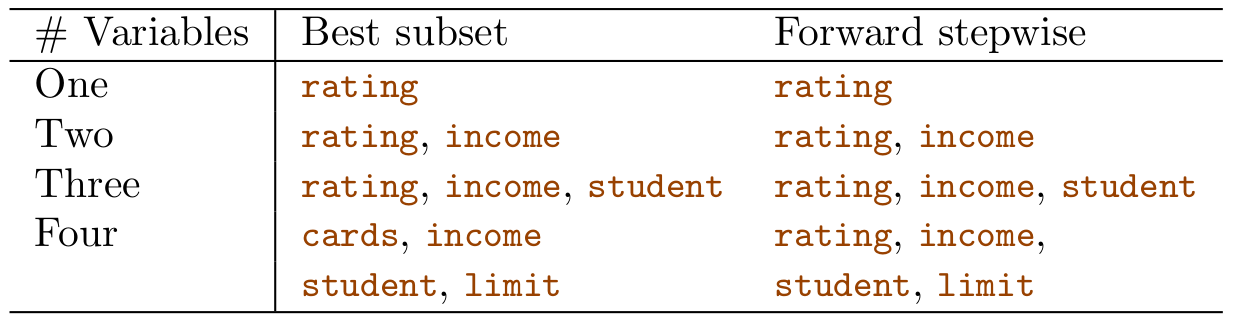
\includegraphics[width = \textwidth, align = c]{Table6-1}


% \end{columns}
% \InstructorList{
% \item Again on \texttt{Credit} data set
% \item First three models are the same, but the fourth is different
% \item Going back to figure of $R^2$, we can check that score was similar so it's ok
% }

% \end{frame}
%--- Next Frame ---%
%=================
\section{Backward Selection}
%=================

\begin{frame}[c]{Backward stepwise selection}

\begin{columns}
\column{.65\textwidth}
\centering
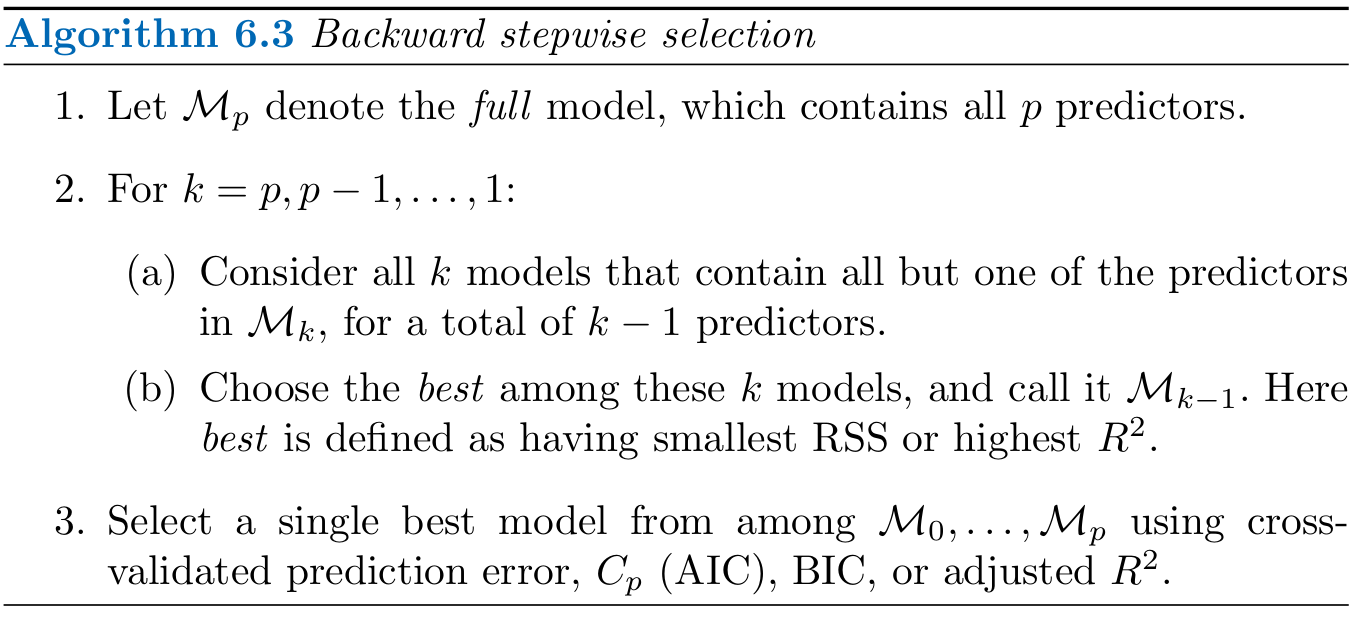
\includegraphics[width = \textwidth, align = c]{Alg6-3}

\end{columns}

\end{frame}
%--- Next Frame ---%
% \begin{frame}[c]{An example for Backward Stepwise Selection}

% 	\centering
% % All subsets of 4 variables ($2^4 = 16$)

% \begin{columns}
% \column{.2\textwidth}
% \centering
% \begin{itemize}
% 	\item $\emptyset$
% \end{itemize}
% \column{.2\textwidth}
% \centering

% \begin{itemize}
% 	\item $X_1$
% 	\item $X_2$
% 	\item $X_3$
% 	\item $X_4$
% \end{itemize}
% \column{.2\textwidth}
% \centering
% \begin{itemize}
% 	\item $X_1$ $X_2$
% 	\item $X_1$ $X_3$
% 	\item $X_1$ $X_4$
% 	\item $X_2$ $X_3$
% 	\item $X_2$ $X_4$
% 	\item $X_3$ $X_4$
% \end{itemize}
% \column{.2\textwidth}
% \centering
% \begin{itemize}
% 	\item $X_1$ $X_2$ $X_3$
% 	\item $X_1$ $X_2$ $X_4$
% 	\item $X_1$ $X_3$ $X_4$
% 	\item $X_2$ $X_3$ $X_4$
% \end{itemize}
% \column{.2\textwidth}
% \centering
% \begin{itemize}
% 	\item $X_1$ $X_2$ $X_3$ $X_4$
% \end{itemize}
% \end{columns}
% \end{frame}
% %--- Next Frame ---%
% {
% \setbeamercolor{background canvas}{bg=Apricot!25}
% \begin{frame}[t]{Group work: by hand same example with backward}
% We train a model using four variables, $X_1,X_2,X_3,X_4$.
% We're interested in getting a subset of the variables to use. The following table shows the mean squared error and the $R^2$ value computed for the model learned using each possible subset of variables.
% \begin{columns}
% \column{.45\textwidth}
% \centering
% % \begin{wrapfigure}{r}{1in}
% \begin{center}
% 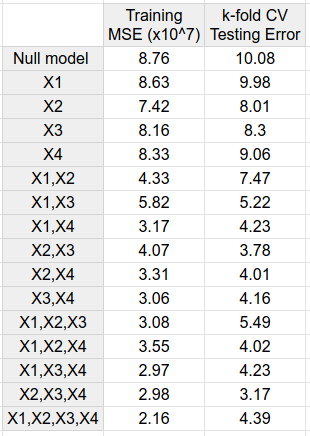
\includegraphics[width = .5\textwidth]{FakeData-SubsetSelection.png}
% \end{center}
% % \end{wrapfigure}

% \column{.45\textwidth}
% \centering
% \begin{enumerate}
% %   \item What subset of variables is found for each of the sets $\mathcal{M}_0,\mathcal{M}_1,\mathcal{M}_2,\mathcal{M}_3,\mathcal{M}_4$ when using best subset selection?
% % \vfill
% %   \item What subset of variables is returned using best subset selection?

% % \vfill
%   \item What subset of variables is found for each of the sets $\mathcal{M}_0,\mathcal{M}_1,\mathcal{M}_2,\mathcal{M}_3,\mathcal{M}_4$ when using forward selection?
% \vfill
%   \item What subset of variables is returned using forward subset selection?
% \vfill
% \end{enumerate}

% \end{columns}
% \end{frame}
% }
% %----Next frame-----%
% {
% \setbeamercolor{background canvas}{bg=Apricot!25}
% \begin{frame}[t]{Extra work space if it helps}
% \begin{columns}
% \column{.25\textwidth}
% 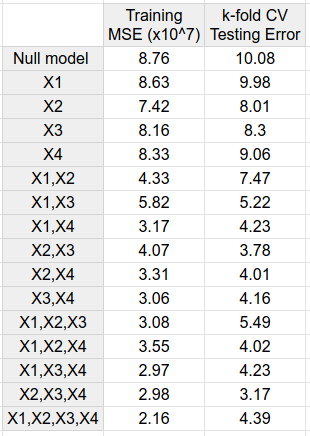
\includegraphics[width = \textwidth]{FakeData-SubsetSelection.png}

% \centering
% \column{.1\textwidth}
% \centering
% \begin{itemize}
% 	\item $\emptyset$
% \end{itemize}
% \column{.1\textwidth}
% \centering

% \begin{itemize}
% 	\item $X_1$
% 	\item $X_2$
% 	\item $X_3$
% 	\item $X_4$
% \end{itemize}
% \column{.15\textwidth}
% \centering
% \begin{itemize}
% 	\item $X_1$ $X_2$
% 	\item $X_1$ $X_3$
% 	\item $X_1$ $X_4$
% 	\item $X_2$ $X_3$
% 	\item $X_2$ $X_4$
% 	\item $X_3$ $X_4$
% \end{itemize}
% \column{.15\textwidth}
% \centering
% \begin{itemize}
% 	\item $X_1$ $X_2$ $X_3$
% 	\item $X_1$ $X_2$ $X_4$
% 	\item $X_1$ $X_3$ $X_4$
% 	\item $X_2$ $X_3$ $X_4$
% \end{itemize}
% \column{.2\textwidth}
% \centering
% \begin{itemize}
% 	\item $X_1$ $X_2$ $X_3$ $X_4$
% \end{itemize}
% \end{columns}
% \InstructorNotes{
% $
% \mathcal{M}_0 = \emptyset,
% \mathcal{M}_1 = \{X_3\},\,
% \mathcal{M}_2= \{X_3,X_4\},\,
% \mathcal{M}_3= \{X_1,X_3,X_4\},\,
% \mathcal{M}_4 = \{X_1,X_2,X_3,X_4\},\,$.\\
%  Among test error, best is  $X_3X_4$}
% \end{frame}
% }
% %--- Next Frame ---%
%--- Next Frame ---%

\begin{frame}[t]{Pros and Cons of Backward Stepwise}

\begin{columns}
\column{.45\textwidth}
\centering
\textbf{Pros:}

\InstructorList{
\item Computationally cheaper
\item Number of models fit is still
\begin{equation*}
	1 + \sum_{k=0}^{p-1} (p-k) = 1 + \frac{p(p+1)}{2}
\end{equation*}
which is way better than $2^p$
}
\column{.45\textwidth}
\centering
\textbf{Cons:}

\InstructorList{
\item Not guaranteed to find the best model
\item Unlike forward selection, this can't be used at all if $n<p$
}

\end{columns}
\InstructorNotes{Can also look at hybrid approaches with both forward and backward selection}
\end{frame}
%--- Next Frame ---%


% %==========
% \section{Alternatives for Approximating Test Error}
% %==========
% \begin{frame}[c]{Remembering what we're doing}

% \begin{columns}
% \column{.45\textwidth}
% \centering
% 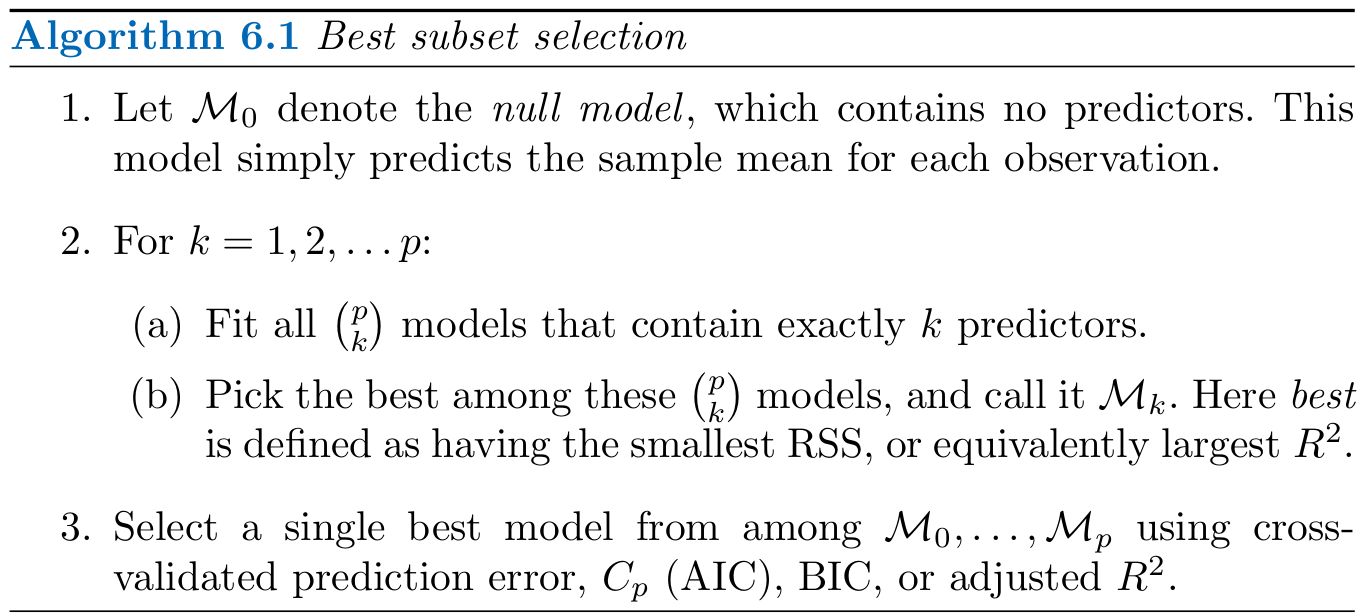
\includegraphics[width = \textwidth, align = c]{Alg6-1}
% \InstructorNotes{Now we're focusing on step 3}
% \column{.45\textwidth}
% \centering
% 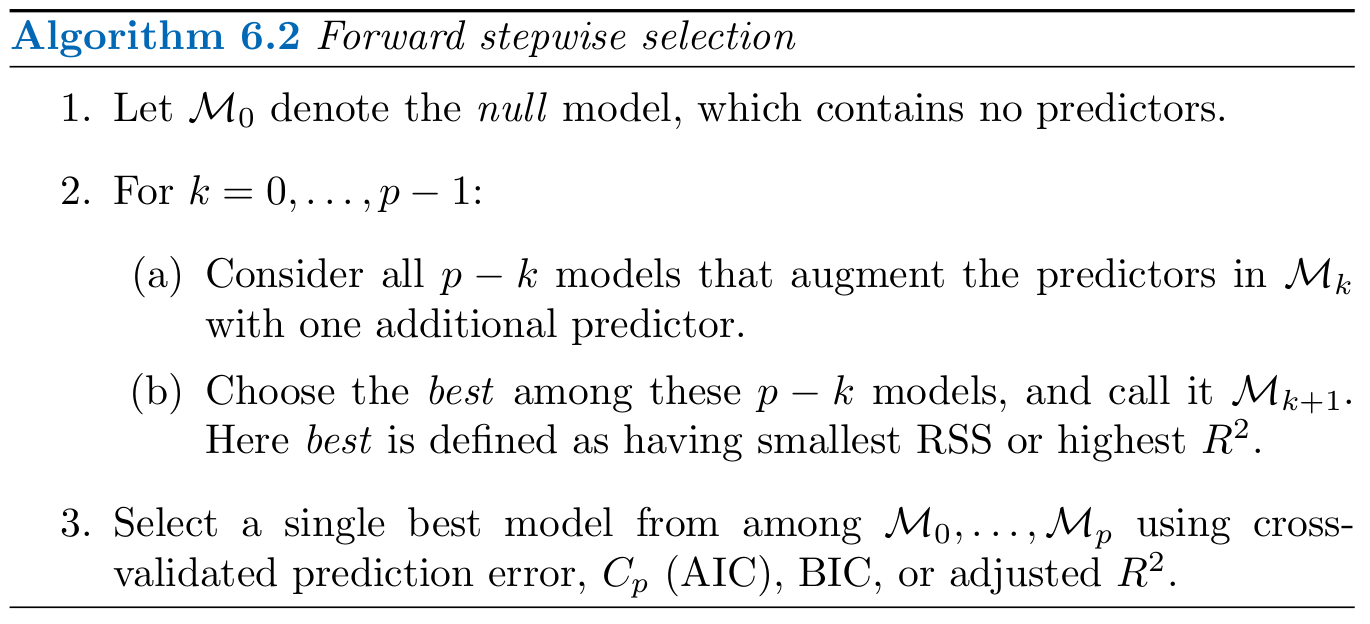
\includegraphics[width = \textwidth, align = c]{Alg6-2}
% 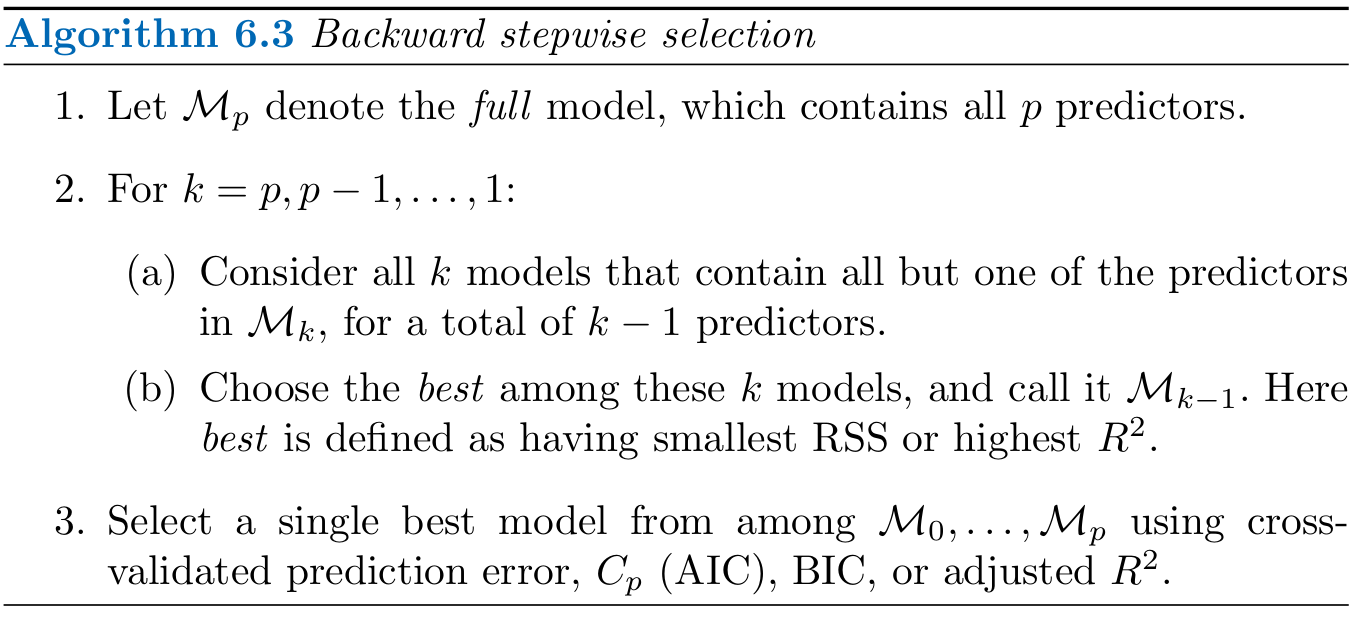
\includegraphics[width = \textwidth, align = c]{Alg6-3}

% \end{columns}
% \InstructorNotes{The goal is to come up with ways to adjust the training scores to get something that better approximates testing scores}
% \end{frame}
% %--- Next Frame ---%
% \begin{frame}[t]{The $C_p$ estimate}

% 	\begin{equation*}
% 		C_p = \frac{1}{n}(\mathrm{RSS} + 2 d \hat \sigma^2)
% 	\end{equation*}



% \begin{columns}
% \column{.2\textwidth}
% \centering
% 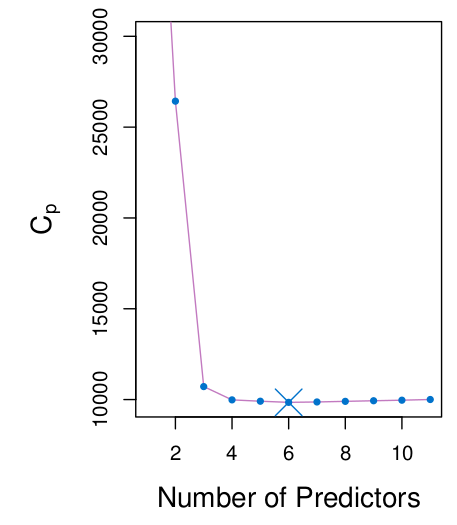
\includegraphics[width = \textwidth, align = c]{Fig6-2a}
% Example using \texttt{Credit}
% \column{.3\textwidth}
% \centering
% \InstructorList{
% \item The $p$ does nothing. It's not our usual $p$. WTF
% \item $d$ is the number of predictors you're using to fit
% \item $\hat \sigma^2$ is an estimate of $\Var(\e)$
% }
% \column{.45\textwidth}
% \centering
% \InstructorList{
% \item Penalty increases with more $d$, so aims for fewer predictors
% \item This acts to adjust for the overfitting decrease in RSS from higher $d$
% \item One can show that if $\hat \sigma^2$ is an unbiased estimate of $\sigma^2$, then $C_p$ is an unbiased estimate of test MSE.
% \item So.... aim for model with lowest $C_p$
% \item This example takes a 6 variable model
% }
% \end{columns}

% \end{frame}
% %--- Next Frame ---%
% \begin{frame}[t]{The AIC criterion}

% 	\begin{equation*}
% 		\mathrm{AIC} = \frac{1}{n}(\mathrm{RSS}+2d\hat \sigma^2)
% 	\end{equation*}



% \begin{columns}
% \column{.2\textwidth}
% \centering
% 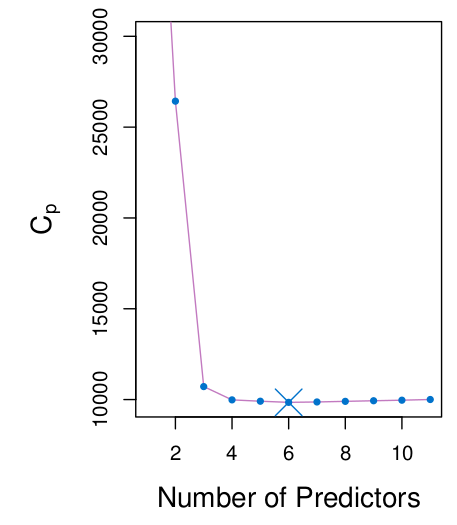
\includegraphics[width = \textwidth, align = c]{Fig6-2a}
% Example using \texttt{Credit}
% \column{.3\textwidth}
% \centering
% \InstructorList{
% \item Works for large class of models fit by maximum likelihood
% \item Dropping the constants phrase is doing a lot of work, but means $C_p$ and AIC proportional
% \item $C_p$ and AIC are proportional, so only draw $C_p$ here
% }
% \column{.45\textwidth}
% \centering
% \end{columns}

% \end{frame}
% %--- Next Frame ---%
% \begin{frame}[t]{The BIC}
% 	\begin{equation*}
% 		\mathrm{BIC} = \frac{1}{n}(\mathrm{RSS}+\log(n)d\hat \sigma^2)
% 	\end{equation*}

% 	\begin{columns}
% 	\column{.2\textwidth}
% 	\centering
% 	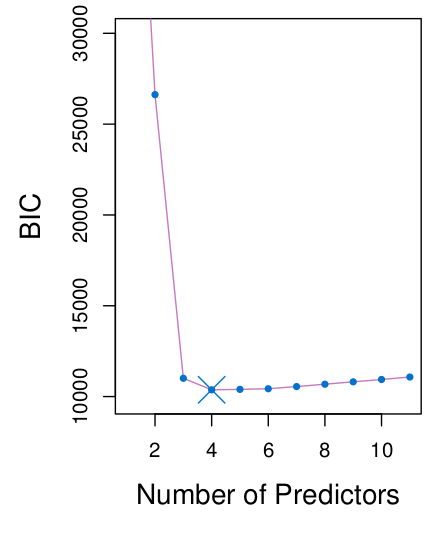
\includegraphics[width = \textwidth, align = c]{Fig6-2b}
% 	Example using \texttt{Credit}
% 	\column{.3\textwidth}
% 	\centering
% 	\InstructorList{
% 	\item Dervied from Baysean statistics
% 	\item $\log(n) >2$ if $n>7$, so heavier penalty on models with many variables than $C_p$
% 	}
% 	\column{.45\textwidth}
% 	\centering
% 	\end{columns}


% \end{frame}
% %--- Next Frame ---%
% \begin{frame}[t]{Adjusted $R^2$}

% \begin{columns}
% \column{.45\textwidth}
% \centering
% \begin{equation*}
% 	R^2 = 1-\frac{\mathrm{RSS}}{\mathrm{TSS}}
% \end{equation*}
% \column{.45\textwidth}
% \centering

% \begin{equation*}
% \text{adjusted }	R^2 = 1-\frac{\mathrm{RSS}/(n-d-1)}{\mathrm{TSS}/(n-1)}
% \end{equation*}
% \end{columns}


% \begin{columns}
% \column{.2\textwidth}
% \centering
% 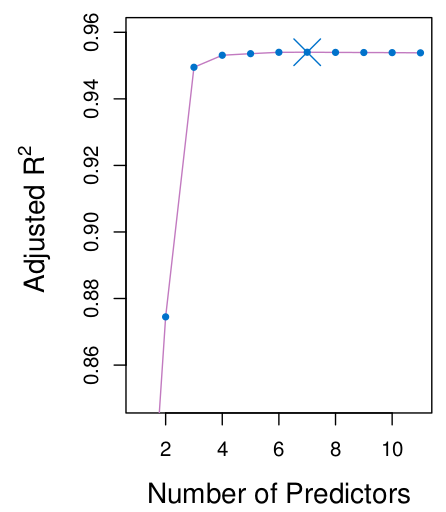
\includegraphics[width = \textwidth, align = c]{Fig6-2c}
% \column{.3\textwidth}
% \centering
% \InstructorList{
% \item $TSS = \sum (y_i - \bar y)^2$ total sum of squares
% \item A large value means small test error, so we want the $R^2$ to go up
% \item $RSS$ always decreases as number of variables increases, but $RSS/(n-d-1)$ could go up or down.
% }
% \column{.45\textwidth}
% \centering
% \InstructorList{
% \item Idea is that including additional variables to the model that are noise leads to small decrease in RSS.
% \item In that case, $d$ always up by 1, so $\frac{RSS}{n-d-1}$ will increase, causing $R^2$ to decrease
% \item View this as penalizing adding unnecessary variables
% }
% \end{columns}


% \end{frame}
% %--- Next Frame ---%
% \begin{frame}[c]{Comparisons}

% \begin{columns}
% \column{.45\textwidth}
% \centering
% \InstructorList{
% \item $C_p$, AIC, BIC have rigorous justifications that we're gonna skip
% \item $R^2$ is intuitive, but doesn't really come with theoretical justification
% \item These equations presented are in the case of least squares fit. AIC and BIC have versions that can be defined in the case of more general models
% }
% \column{.45\textwidth}
% \centering

% \end{columns}

% \end{frame}
% %--- Next Frame ---%
% \begin{frame}[t]{All this vs.~Validation and Cross Validation}
% \centering
% 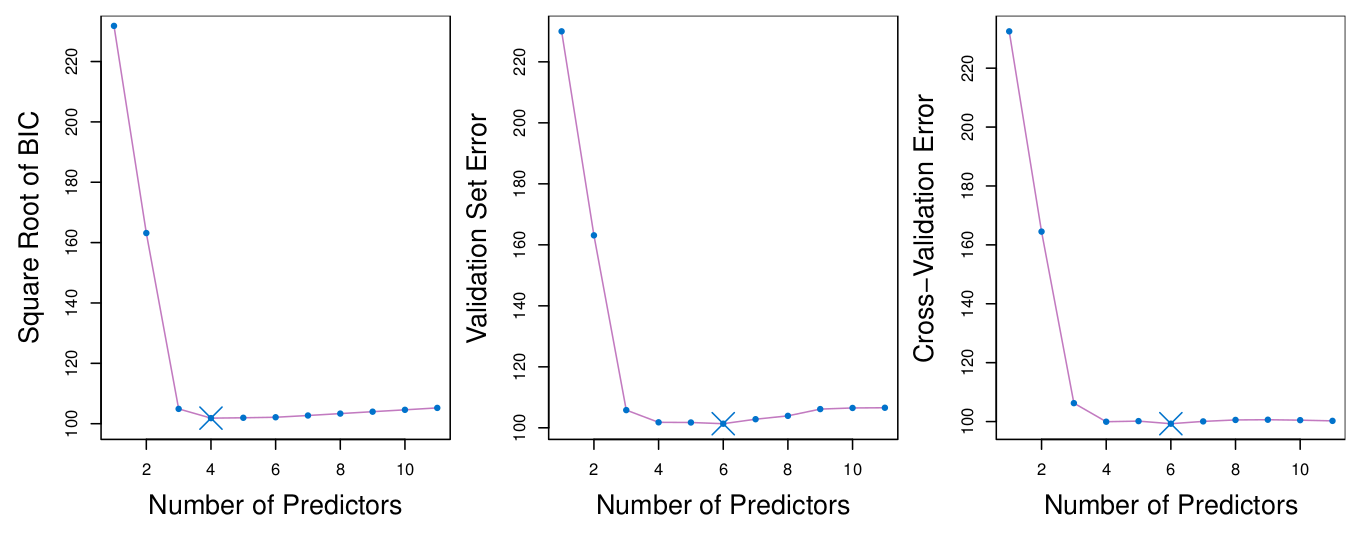
\includegraphics[width = .7\textwidth, align = c]{Fig6-3}
% \begin{columns}
% \column{.45\textwidth}
% \centering
% \footnotesize
% \InstructorList{
% \item The goal was to approximate test error, so why not do validation or CV instead?
% \item Historically, CV was computationally prohibitive. These tools were an alternative to deal with the same question but with much cheaper computation
% }
% \column{.45\textwidth}
% \centering
% \InstructorList{
% \item All versions show 3,4,5 are basically equivalent choices
% \item
% }

% \end{columns}

% \end{frame}
%--- Next Frame ---%
\begin{frame}[c]{TL;DR}

\begin{columns}
\column{.55\textwidth}
\centering
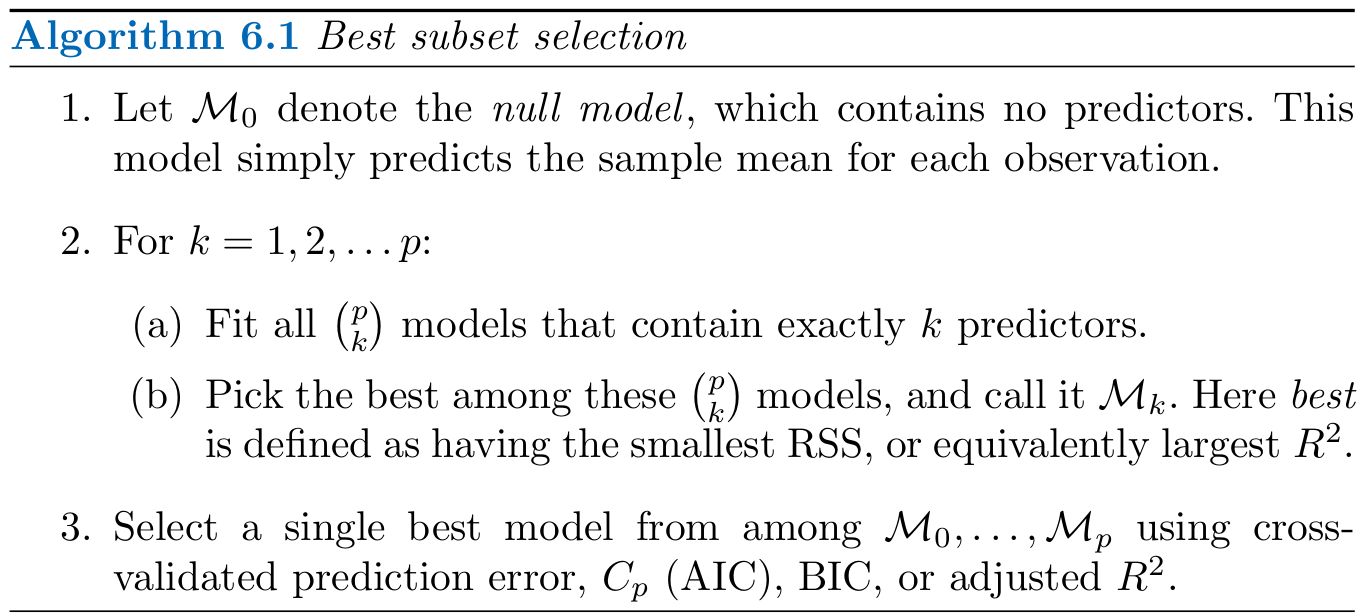
\includegraphics[width = \textwidth, align = c]{Alg6-1}
\column{.35\textwidth}
\centering
\begin{itemize}
	\item Modify step 2 with forward or backward selection
	\item Choose best model in step 3 using one of our adjusted training scores or CV
\end{itemize}

\end{columns}
\vfill

\end{frame}
%--- Next Frame ---%
% %----------------
\begin{frame}[t]{Next time}


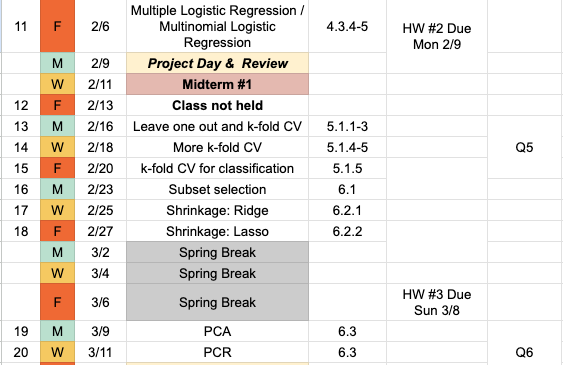
\includegraphics[align = c, width = .65\textwidth]{Schedule-S26-Lecs11_to_20}


\end{frame}
%--- Next Frame ---%


\end{document}
